\documentclass{article}

\usepackage{neurips_2023}
\usepackage[utf8]{inputenc}
\usepackage[T1]{fontenc}
\usepackage[hidelinks]{hyperref}
\usepackage{url}
\usepackage{booktabs}
\usepackage{amsfonts}
\usepackage{nicefrac}
\usepackage{microtype}
\usepackage{xcolor}
\usepackage{graphicx}
\usepackage{amsmath,amssymb}
\usepackage{algorithm}
\usepackage{algorithmic}
\usepackage{enumitem}
\usepackage[table]{colortbl}
\usepackage{multirow}
\usepackage{wrapfig}

% Colors from Struct Memory-R1 figure palette
\definecolor{clrMgr}{HTML}{56669E}      % Memory Manager indigo
\definecolor{clrRet}{HTML}{728AB9}      % Retrieval Agent steel blue
\definecolor{clrAns}{HTML}{CEA2B5}      % Answer Agent dusty rose
\definecolor{clrOk}{HTML}{50B9AE}       % Success teal
\definecolor{clrStruct}{HTML}{9A9AB9}   % Structure lavender
% Light tints for table headers
\definecolor{hdrOverall}{HTML}{E0F0ED}  % light teal
\definecolor{hdrMH}{HTML}{E8EAF2}      % light indigo
\definecolor{hdrSH}{HTML}{F5E8EE}      % light rose
\definecolor{hdrTemp}{HTML}{EDEAF5}     % light lavender
\definecolor{hdrOD}{HTML}{E8F0F8}      % light steel blue
\definecolor{rowOurs}{HTML}{E8F8F5}     % very light teal for our row
\definecolor{rowOracle}{HTML}{F5F5F5}   % very light gray for oracle

\title{\textsc{Struct Memory-R1}: Long-Horizon Conversational Memory Access and Updates over Tree-Structured Memory with Reinforcement Learning}

\author{
  Yifan Liu \And Liam Gallagher \And David Courtis \And Jiazhou Liang
}

\begin{document}

\maketitle

\begin{abstract}
AI agents must maintain long-horizon memory over conversational history to provide relevant context for future interactions. We observe that conversational information has natural event and topic based structure that a tree can capture. Once memory is a tree, however, access and updates work differently from their flat counterparts: the retriever must select branches before reading leaves, and the writer must decide where in the hierarchy new facts belong. Both access and updates now involve reasoning through possible trajectories in the tree, and whether the chosen path is correct can only be judged by the final answer to a future question. We propose \textsc{Struct Memory-R1}, a framework that induces tree-structured memory from raw conversation and uses reinforcement learning from question-answering reward to train three components: a \emph{Memory Manager} for tree updates, a \emph{Retrieve Agent} for tree access, and an \emph{Answer Agent} for downstream evaluation. On the LoCoMo benchmark, \textsc{Struct Memory-R1} achieves the highest overall F1 and LLM-judge accuracy among non-oracle methods, with particularly large gains on multi-hop (+8.6 F1) and temporal (+14.1 F1) questions over the flat-memory Memory-R1 baseline.
\end{abstract}

\section{Introduction}

\begin{wrapfigure}{r}{0.5\textwidth}
\vspace{-18pt}
\centering
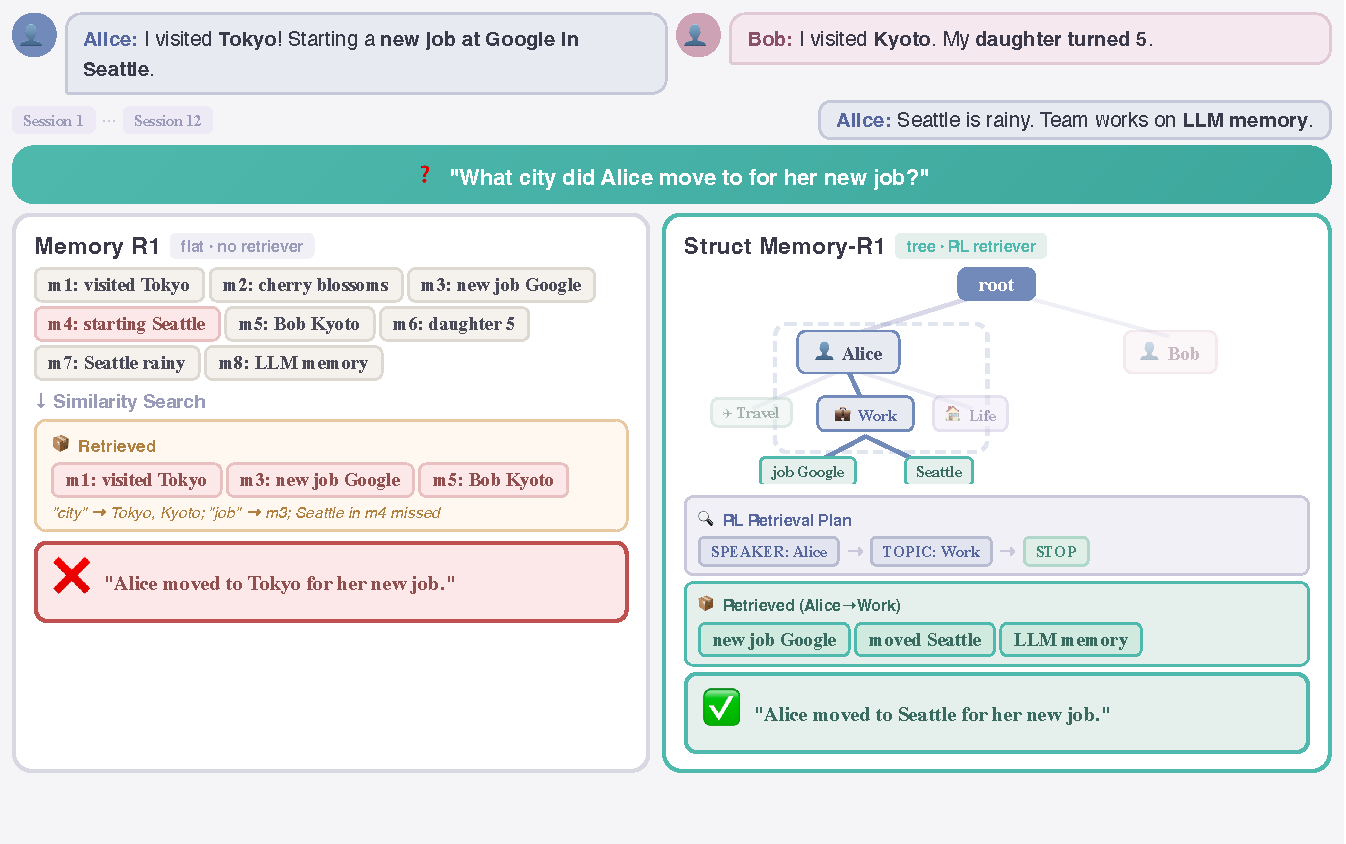
\includegraphics[width=0.5\textwidth]{figures/hook_figure.pdf}
\caption{{Motivating example.} \textbf{Memory R1} (left) uses flat similarity search, retrieving ``Tokyo'' for ``city'' but missing the job--Seattle link. \textbf{Struct Memory-R1} (right) navigates Alice $\rightarrow$ Work in the tree, correctly finding ``Seattle.''}
\label{fig:hook}
\vspace{-10pt}
\end{wrapfigure}

Memory-augmented large language models (LLMs) maintain an external memory bank that stores information from past interactions and retrieves relevant context to condition future responses~\cg{zhang2024survey}. This paradigm enables long-horizon conversational agents to access information beyond the fixed context window~\cg{maharana2024evaluating}. However, most existing memory systems represent memories as flat, unordered collections and rely on similarity-based retrieval to access them~\cg{lewis2020retrieval, khandelwal2020generalization, park2023generative}.

Flat retrieval treats all memories as independent entries in a global scoring space, ignoring the inherent relationships among them. When a user's history spans dozens of sessions covering multiple topics, events, and evolving facts, scoring each memory independently leads to \emph{retrieval interference}---semantically similar but contextually irrelevant entries compete with the correct ones. Flat update mechanisms, whether append or overwrite, similarly lack structural awareness: when a new fact arrives, the system cannot determine whether it extends an existing topic or introduces a new one. As conversations grow, these limitations compound, making consistent memory maintenance increasingly difficult.

Conversational information, however, has natural hierarchical structure: discussions revolve around people and topics, topics unfold through events and sessions, and individual facts exist within these groupings. A tree captures this hierarchy, enabling retrieval to first select a relevant branch and then read the leaves within it, and enabling updates to place new facts relative to their structural neighbors rather than into a global pool. Several prior works have explored tree-structured memory representations, including MemTree~\cg{rezazadeh2024memtree}, RAPTOR~\cg{sarthi2024raptor}, Lattice~\cg{lattice2025}, and MemWalker~\cg{chen2023memwalker}. These methods rely on heuristic or LLM-prompted approaches to construct and traverse memory hierarchies.

However, both access and update over a tree involve \emph{reasoning} through possible trajectories: the retriever must decide which branches to explore, and the writer must decide where a new fact belongs in the hierarchy (\autoref{fig:hook}). The quality of these intermediate decisions can only be judged by the correctness of the downstream answer, and direct supervision for such decisions is unavailable in standard QA data. Reinforcement learning from downstream question-answering reward is therefore the natural training signal. This follows the principle established by Search-R1~\cg{jin2025search} and Memory-R1~\cg{yan2025memory}---that information access should be trained from task outcomes---and extends it from flat memory to tree-structured access and updates.

We therefore propose \textsc{Struct Memory-R1}, a reinforcement-learning framework that learns tree-structured conversational memory from raw interaction history. \textsc{Struct Memory-R1} decomposes the problem into three coordinated components (\autoref{fig:overview}):
\begin{itemize}[nosep,leftmargin=1.5em]
\item A \textbf{Memory Manager} that receives a new turn and the current memory, then incrementally constructs and updates the memory tree through structural placement of new facts.
\item A \textbf{Retrieve Agent} that operates over the induced tree and emits an explicit search plan, selecting branches and leaves rather than relying on global flat retrieval.
\item An \textbf{Answer Agent} that reads retrieved evidence and produces the final answer.
\end{itemize}

\begin{figure}[t]
\centering
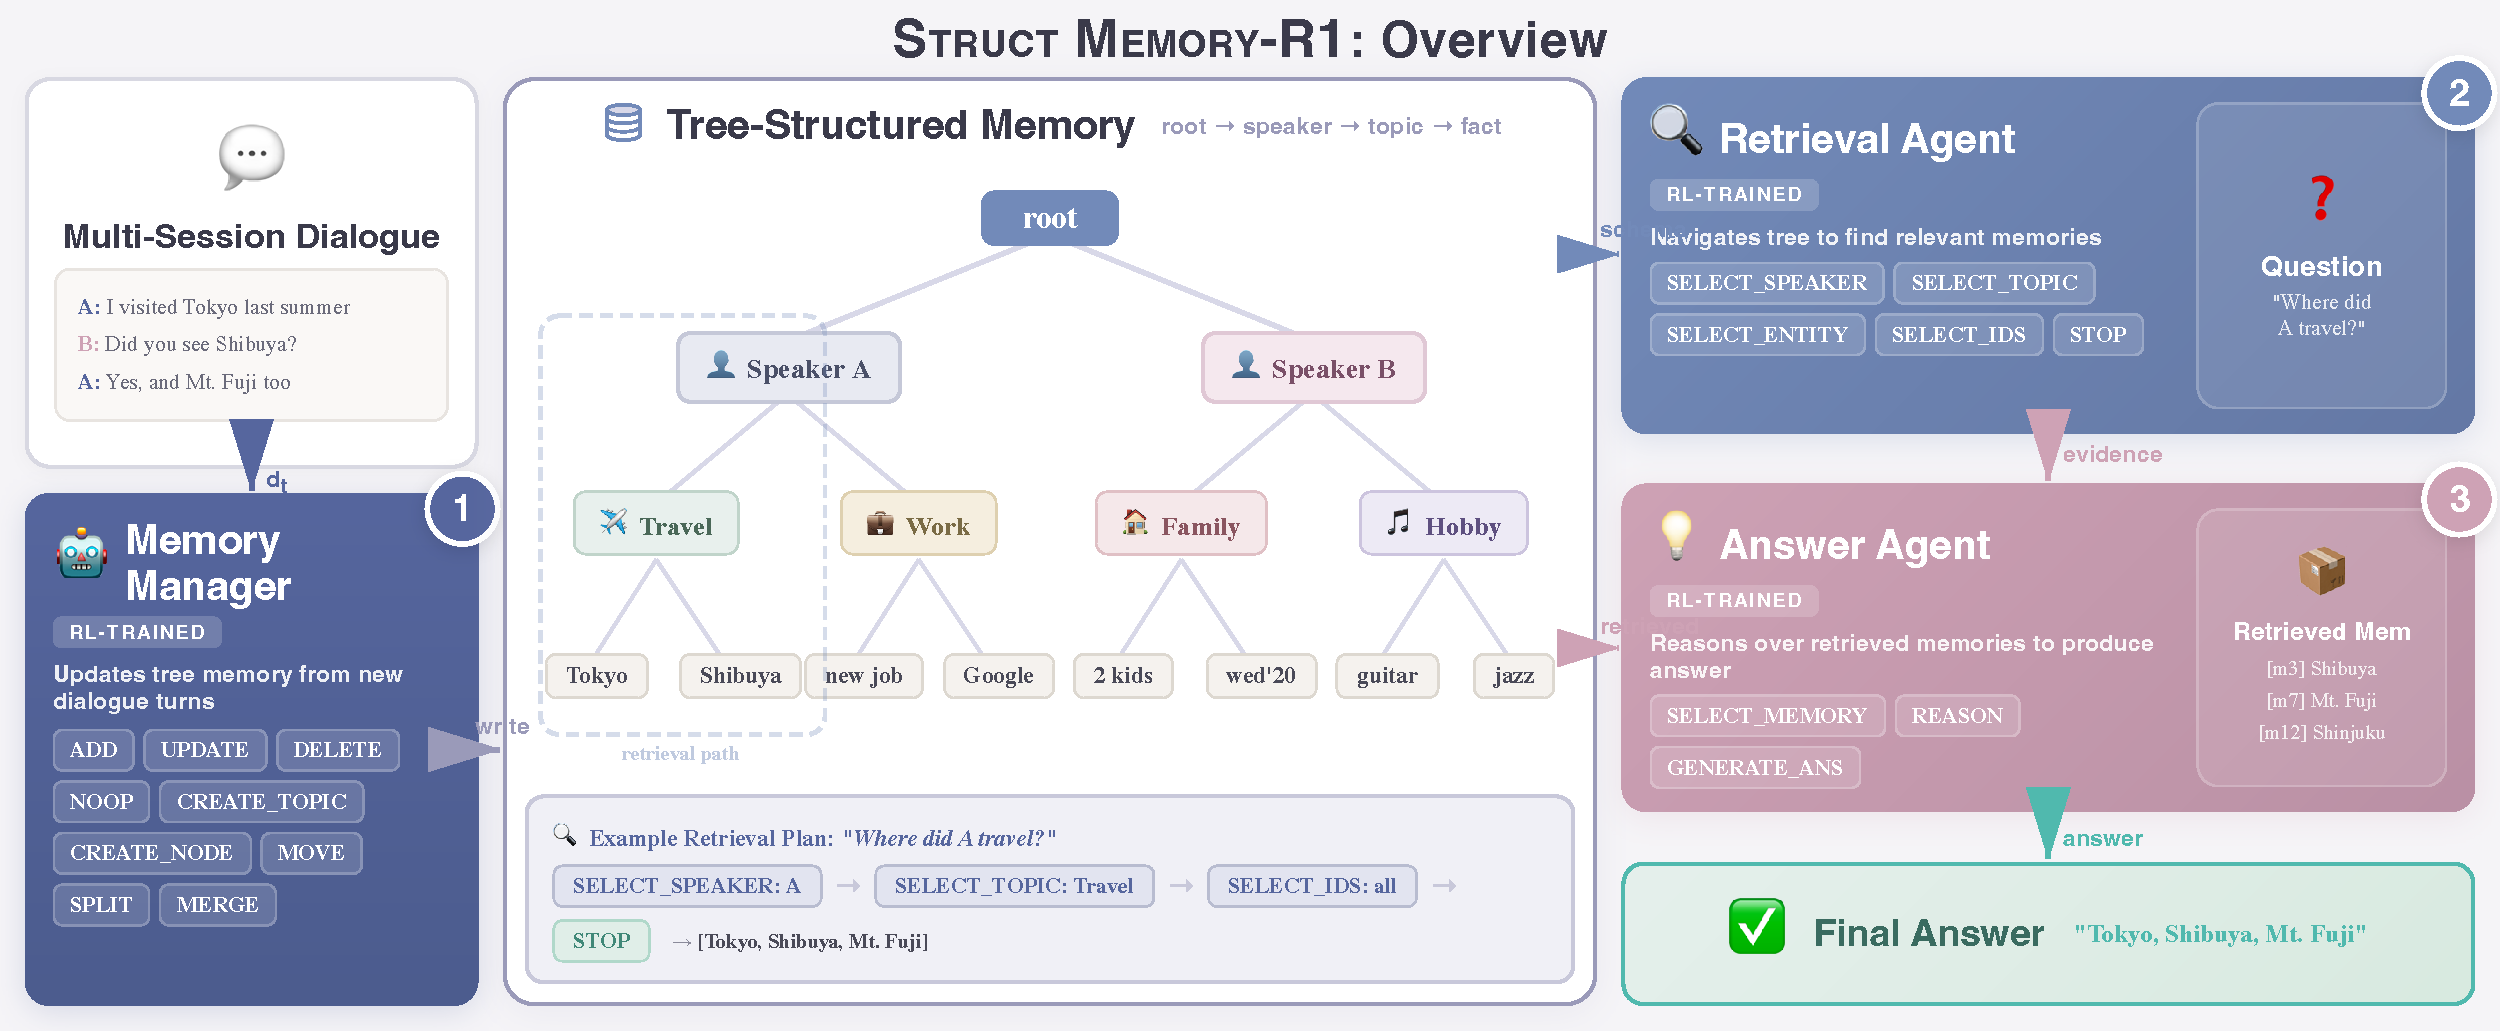
\includegraphics[width=\textwidth]{figures/struct_memory_r1_figure.pdf}
\caption{{Overview of \textsc{Struct Memory-R1}.} The Memory Manager induces and updates a tree-structured memory from raw conversation. The Retrieve Agent emits a search plan over the tree to select relevant evidence. The Answer Agent produces the final response. All three components are trained with reinforcement learning from downstream question-answering reward.}
\label{fig:overview}
\end{figure}

The decomposition follows the causal chain of the problem: the Memory Manager builds and maintains the tree, the Retrieve Agent navigates it for a given question, and the Answer Agent evaluates whether the retrieved evidence suffices. By separating these roles, \textsc{Struct Memory-R1} turns structured memory into a modular reinforcement-learning problem in which tree updates, tree access, and answering are each optimized via Group Relative Policy Optimization (GRPO) against downstream task performance.

In summary, the paper makes three contributions:
\begin{itemize}[nosep,leftmargin=1.5em]
\item We formalize the memory-augmented LLM setting and argue that conversational memory has hierarchical structure that a tree captures naturally, requiring access and update operations that differ fundamentally from those used on flat memory.
\item We propose \textsc{Struct Memory-R1}, a three-component framework that induces tree structure from raw conversation and trains tree-specific access and update policies with GRPO-based reinforcement learning.
\item We evaluate on the LoCoMo benchmark~\cg{maharana2024evaluating}, showing that tree-structured memory yields substantial gains on multi-hop (+9.0 F1) and temporal (+13.8 F1) questions while achieving the highest overall F1 among non-oracle methods.
\end{itemize}

\section{Problem Definition}
(todo: this section is not good). i want you to focus on memory augmented LLM. where you have LLM, which take external memory to answer question. very formally and mathmatically. 
\paragraph{Conversational Agent.}

We consider an LLM-based agent augmented with an external memory system that persists across interactions:
\begin{equation}
\mathcal{A} = (\pi_\theta,\; \mathcal{X},\; \mathcal{Y},\; \mathcal{M},\; \mathcal{E}),
\end{equation}
\begin{itemize}[nosep]
    \item \textbf{policy} $\pi_\theta$: maps an observation and a memory state to a distribution over action trajectories;
    \item \textbf{input (observation) space}  $\mathcal{X}$: the set of all possible user queries and dialogue the agent may receive;
    \item \textbf{output (response) space} $\mathcal{Y}$ : the set of all possible natural-language responses the agent may produce;
    \item  \textbf{memory space} $\mathcal{M}$: the set of all possible external memory states the agent can read from and write to;
    \item \textbf{external environment interface} $\mathcal{E}$: the set of tools through which the agent can perform actions beyond pure language generation (e.g., a memory retrieval server, a search engine, or a code executor).
\end{itemize}


An \emph{interaction} is a temporally ordered sequence of turns between a user and the agent:
\begin{equation}
\mathcal{I} = (t_1, t_2, \ldots, t_T),
\end{equation}
where $T$ is the total number of turns in the interaction.
At turn $t$ ($1 \le t \le T$), the user provides an input $x_t \in \mathcal{X}$ (a query, instruction, or follow-up). The agent observes $x_t$ together with the current memory state $M_t \in \mathcal{M}$. T

The agent generates an action trajectory as a sequence of \emph{language actions} (reasoning steps, final answers) and \emph{environment actions} (memory queries, tool calls).
The agent emits a final response $y_t \in \mathcal{Y}$ extracted from $\tau_t$. The memory state may be updated: $M_{t+1} = f_{\text{update}}(M_t, \tau_t)$, where $f_{\text{update}}$ encodes any write operations performed during the turn.
The objective is to learn a policy $\pi_\theta$ that controls memory access when and how memory should be queried to improve downstream task performance. 

\paragraph{Memory Structures}

Recent work, notably Search-R1~\citep{jin2025search}  and Memory-R1~\citep{yan2025memory}\footnote{Memory-R1 does not provide a public codebase. We built a publicly available implementation at \url{https://github.com/YifanLiu2/Struct_Memory_R1.git}.}, has shown that RL can effectively train agents to manage flat external memory banks.
A \emph{flat memory state} is an unordered collection of $N$ memory entries:
\begin{equation}
M_t^{\text{flat}} = \{m_1, m_2, \ldots, m_N\}, \quad m_i = (\text{key}_i,\; \text{attributes}_i),
\end{equation}
\section{Method}

\subsection{Overview}
\textsc{Struct Memory-R1} instantiates the memory-augmented LLM framework defined in Section~2 with three learned components: a Memory Manager $\pi_{\theta_M}$, a Retrieve Agent $\pi_{\theta_R}$, and an Answer Agent $\pi_{\theta_A}$. Each component is parameterized by a language model and trained with Group Relative Policy Optimization (GRPO)~\cg{shao2024deepseekmath} using downstream question-answering reward. Training proceeds in stages: the Answer Agent is trained first, then frozen while the Retrieve Agent and Memory Manager are trained in sequence. This staged approach ensures stable reward signals at each phase.

\subsection{Memory Bank and Tree Structure}
The memory bank $\mathcal{T}_t = (V_t, E_t)$ is a rooted tree that is constructed incrementally from raw conversation. Each node $v \in V_t$ resides at a level $\ell(v) \in \{0, 1, \ldots, L\}$ and carries content $c(v)$. The tree is structured such that:
\begin{itemize}[nosep,leftmargin=1.5em]
\item Level 0: the root, representing the full conversation;
\item Levels $1$ to $L{-}1$: internal nodes representing hierarchical groupings (e.g., people, topics, events);
\item Level $L$: leaf nodes, each containing an individual memory entry $m_i$.
\end{itemize}
Each internal node $v$ maintains a summary $s(v)$ that aggregates information from its children $\text{Ch}(v) = \{u \in V_t : (v, u) \in E_t\}$. The \emph{schema} of the tree, $\textsc{Schema}(\mathcal{T}_t)$, consists of node identifiers and summaries at each level without exposing full leaf content, providing a compact representation for the retrieval policy.

The tree is serialized as structured JSON for input to language model policies. This serialization preserves the hierarchical relationships while remaining compatible with standard text-based LLM input formats.

\subsection{Memory Manager}
The Memory Manager observes the current dialogue turn $x_t$ and the current memory tree $\mathcal{T}_t$, and emits a set of operations to update the tree. We restrict the operation space to four stable CRUD operations:
\begin{equation}
\mathcal{O} = \{\textsc{Add}, \textsc{Update}, \textsc{Delete}, \textsc{None}\}.
\end{equation}
Given turn $x_t$ and tree $\mathcal{T}_t$, the manager samples an operation sequence:
\begin{equation}
o_t \sim \pi_{\theta_M}(\cdot \mid x_t, \mathcal{T}_t),
\end{equation}
and the updated tree is obtained deterministically:
\begin{equation}
\mathcal{T}_{t+1} = \textsc{Apply}(\mathcal{T}_t, o_t).
\end{equation}
The operation $o_t$ is a JSON object specifying which entries to add, modify, or remove, along with their placement in the tree hierarchy. By restricting to CRUD operations rather than arbitrary structural rewrites, we isolate the benefit of structured memory from the complexity of unrestricted topology editing.

\paragraph{Reward.}
The Memory Manager is trained with outcome-driven reward. After applying the manager's operations, the downstream pipeline (Retrieve Agent + frozen Answer Agent) processes the corresponding question. The reward is:
\begin{equation}
r_M = \mathcal{R}(y_t, y_t^\star) + \lambda_f \cdot \mathbb{1}[\text{valid JSON}],
\end{equation}
where $\mathcal{R}(y_t, y_t^\star)$ measures answer quality and $\lambda_f$ is a small bonus for well-formed output. This encourages the manager to write memories that are useful for future question answering rather than those matching local heuristics.

\subsection{Retrieve Agent}
The Retrieve Agent operates over the memory tree constructed by the Memory Manager. Given a question $q$ and the tree schema $\textsc{Schema}(\mathcal{T})$, it emits a search plan:
\begin{equation}
z \sim \pi_{\theta_R}(\cdot \mid q, \textsc{Schema}(\mathcal{T})).
\end{equation}
The search plan $z$ is a JSON object of the form:
\begin{equation}
z = \{\texttt{levels}: [\ell_1, \ldots, \ell_k], \;\; \texttt{selected\_ids}: [id_1, \ldots, id_m], \;\; \texttt{stop}: \{0,1\}\},
\end{equation}
where \texttt{levels} specifies which branches to expand at each tree level, \texttt{selected\_ids} names specific leaf nodes to retrieve, and \texttt{stop} terminates search. A deterministic executor runs the plan against the tree:
\begin{equation}
R = \textsc{Execute}(\mathcal{T}, z),
\end{equation}
returning a set of retrieved memory leaves together with local context (parent summaries, sibling information). This design ensures that retrieval is conditioned on structural locality rather than global similarity scoring.

\paragraph{Reward.}
The retriever reward combines answer utility with evidence quality:
\begin{equation}
r_R = \mathcal{R}(y_t, y_t^\star) + \lambda_{\text{ev}} \cdot \textsc{Hit}(R, E^\star) - \lambda_{\text{cost}} \cdot C(z),
\end{equation}
where $E^\star$ denotes gold evidence nodes (when available), $C(z)$ penalizes search cost, and the primary signal is answer quality under a frozen Answer Agent.

\subsection{Answer Agent}
The Answer Agent receives the question $q$ and retrieved memories $R$, and produces a response:
\begin{equation}
y \sim \pi_{\theta_A}(\cdot \mid q, R).
\end{equation}
This component is trained to condition on retrieved evidence rather than on the full conversation history. During Memory Manager and Retrieve Agent training, the Answer Agent is frozen and serves as the evaluator in the reward loop, ensuring that improvements in upstream components are measured through their effect on answer quality.

\subsection{Training with GRPO}
All three components are trained using Group Relative Policy Optimization (GRPO)~\cg{shao2024deepseekmath}, which avoids the need for a separate value network by computing advantages from a group of sampled outputs. For a given input $x$ and policy $\pi_\theta$, GRPO samples a group of $G$ outputs $\{o_1, \ldots, o_G\}$ and computes normalized advantages:
\begin{equation}
\hat{A}_i = \frac{r_i - \mu(\{r_1, \ldots, r_G\})}{\sigma(\{r_1, \ldots, r_G\})},
\end{equation}
where $r_i$ is the reward for output $o_i$, and $\mu, \sigma$ denote the group mean and standard deviation. The policy is updated by maximizing:
\begin{equation}
\mathcal{L}_{\text{GRPO}}(\theta) = \mathbb{E}_{x} \left[ \frac{1}{G} \sum_{i=1}^{G} \min\!\left( \rho_i \hat{A}_i, \; \text{clip}(\rho_i, 1{-}\epsilon, 1{+}\epsilon) \hat{A}_i \right) - \beta \, D_{\text{KL}}\!\left[\pi_\theta \| \pi_{\text{ref}}\right] \right],
\end{equation}
where $\rho_i = \pi_\theta(o_i \mid x) / \pi_{\text{old}}(o_i \mid x)$ is the importance ratio, $\epsilon$ is the clipping parameter, and $\beta$ controls the KL penalty relative to a reference policy $\pi_{\text{ref}}$. This objective encourages the model to produce outputs that yield higher rewards relative to the group average while staying close to the reference distribution.

\section{Experimental Setup}
\subsection{Dataset}
We evaluate on LoCoMo~\cg{maharana2024evaluating}, a long-horizon conversational memory benchmark containing 10 multi-session dialogues with 1{,}540 non-adversarial QA pairs across four question categories: single-hop (282), multi-hop (321), temporal (96), and open-domain (841). We exclude the adversarial category following the Memory-R1 evaluation protocol~\cg{yan2025memory}. Following Memory-R1, we use a 1:1:8 train/validation/test split, yielding 152 training, 81 validation, and 1{,}307 test QA pairs. LoCoMo is well matched to our setting: it requires persistent memory over many turns, supports both single-hop and multi-hop reasoning, and includes temporal and open-domain questions that test different aspects of memory access.

\subsection{Model and Hardware}
All trainable components use Qwen2.5-3B-Instruct as the base policy model. Experiments are run on a single NVIDIA H200 GPU with 16 CPU cores. This setup supports single-node staged GRPO training and fixed-answer-agent evaluation.

We use GRPO as the default policy-optimization method, following Search-R1 and Memory-R1~\cg{jin2025search, yan2025memory}. For the Memory Manager and Retrieve Agent, prompts are formatted as one-shot JSON-generation problems with rule-based reward functions. The Answer Agent is trained to produce short answers conditioned on retrieved memories. During Memory Manager and Retrieve Agent training, the Answer Agent is frozen and used only to compute reward.

\subsection{Baselines}
We organize baselines into three categories.

\paragraph{Context-based.}
\textbf{Full Context} feeds the entire conversation history into the base Qwen2.5-3B-Instruct model without explicit memory or retrieval, relying on the context window alone.
\textbf{Oracle} uses the gold evidence annotations provided in LoCoMo, representing an upper bound on retrieval quality.

\paragraph{Retrieval-based.}
\textbf{RAG (BM25)} applies BM25 keyword retrieval over a flat memory bank of extracted facts.
\textbf{RAG (Embedding)} uses text-embedding-3 dense retrieval over the same flat memory bank.
\textbf{Semantic XPath}~\cg{semanticxpath2026} generates deterministic XPath-style queries over oracle tree-structured memory.

\paragraph{RL-based.}
\textbf{Memory R1}~\cg{yan2025memory} is a flat-memory system with an RL-trained Memory Manager and Answer Agent, trained on the same base model and the same data split for fair comparison.\footnote{Memory-R1 does not provide a public codebase. We built a publicly available implementation at \url{https://github.com/YifanLiu2/Struct_Memory_R1.git}.}

\subsection{Evaluation Metrics}
We report three answer-quality metrics. \textbf{F1} is the token-level F1 score between the predicted and gold answers, measuring lexical overlap. \textbf{B1} is BLEU-1, a unigram precision metric that captures answer conciseness alongside correctness. \textbf{J} is the LLM-as-judge accuracy, where GPT-4o mini evaluates whether the predicted answer is semantically correct given the gold answer. All three metrics are reported per question category (multi-hop, single-hop, temporal, open-domain) and as a weighted overall average reflecting the natural category distribution in LoCoMo.

\section{Results}

\subsection{Main Results}

Table~\ref{tab:main} reports F1, B1, and J across four question categories on the LoCoMo test set.

\begin{table}[t]
\centering
\caption{Main results on LoCoMo (20/80 train/test split, 1{,}232 test QA pairs, adversarial category excluded). F1: token-level F1; B1: BLEU-1; J: LLM-as-judge accuracy (GPT-4o mini). Best non-oracle results per column in \textbf{bold}. Oracle results in \textit{italics}.}
\label{tab:main}
\small
\setlength{\tabcolsep}{2.8pt}
\begin{tabular}{l @{\hskip 5pt} ccc @{\hskip 3pt} ccc @{\hskip 3pt} ccc @{\hskip 3pt} ccc @{\hskip 3pt} ccc}
\toprule
 & \multicolumn{3}{c}{\cellcolor{hdrOverall}\textbf{Overall}} & \multicolumn{3}{c}{\cellcolor{hdrMH}\textbf{Multi-hop}} & \multicolumn{3}{c}{\cellcolor{hdrSH}\textbf{Single-hop}} & \multicolumn{3}{c}{\cellcolor{hdrTemp}\textbf{Temporal}} & \multicolumn{3}{c}{\cellcolor{hdrOD}\textbf{Open-domain}} \\
\textbf{Method} & \cellcolor{hdrOverall}F1 & \cellcolor{hdrOverall}B1 & \cellcolor{hdrOverall}J & \cellcolor{hdrMH}F1 & \cellcolor{hdrMH}B1 & \cellcolor{hdrMH}J & \cellcolor{hdrSH}F1 & \cellcolor{hdrSH}B1 & \cellcolor{hdrSH}J & \cellcolor{hdrTemp}F1 & \cellcolor{hdrTemp}B1 & \cellcolor{hdrTemp}J & \cellcolor{hdrOD}F1 & \cellcolor{hdrOD}B1 & \cellcolor{hdrOD}J \\
\midrule
\multicolumn{16}{l}{\textit{Context-based} \hfill \scriptsize No retrieval; answers from raw context or gold evidence} \\[2pt]
Full Context & 24.2 & 19.7 & 45.7 & 19.7 & 15.8 & 40.4 & 23.9 & 19.0 & 45.7 & 16.2 & 12.5 & 37.3 & 27.0 & 22.3 & 48.6 \\
\rowcolor{rowOracle}Oracle$^\dagger$ & \textit{31.3} & \textit{25.7} & \textit{60.8} & \textit{34.3} & \textit{27.9} & \textit{63.1} & \textit{31.6} & \textit{25.9} & \textit{62.2} & \textit{35.4} & \textit{29.7} & \textit{65.2} & \textit{29.5} & \textit{24.3} & \textit{59.0} \\
\midrule
\multicolumn{16}{l}{\textit{Retrieval-based} \hfill \scriptsize Heuristic or similarity-based retrieval; no RL training} \\[2pt]
RAG (BM25) & 29.9 & 25.3 & 49.8 & 19.0 & 14.6 & 28.1 & 22.6 & 17.6 & 30.6 & 11.2 & 8.8 & 25.1 & \textbf{38.7} & \textbf{33.9} & \textbf{67.3} \\
RAG (Embedding) & 29.5 & 24.3 & 49.6 & 21.1 & 15.8 & 31.5 & 21.8 & 17.3 & 32.4 & 12.1 & 8.8 & 24.2 & 37.2 & 31.7 & 65.1 \\
Semantic XPath & 18.5 & 14.4 & 39.8 & 25.9 & 20.4 & 53.7 & 21.3 & 16.5 & 45.1 & 29.8 & 24.9 & 49.0 & 13.4 & 10.2 & 31.6 \\
\midrule
\multicolumn{16}{l}{\textit{RL-based} \hfill \scriptsize Policy trained with GRPO from downstream QA reward} \\[2pt]
Memory R1 & 27.4 & 22.7 & 53.9 & 22.5 & 17.4 & 50.1 & \textbf{27.7} & \textbf{23.6} & \textbf{54.9} & 20.8 & 16.5 & 48.0 & 30.0 & 25.2 & 55.7 \\
\rowcolor{rowOurs}\textsc{Struct Memory-R1} (Ours)$^*$ & \textbf{30.4} & \textbf{25.4} & \textbf{54.4} & \textbf{31.5} & \textbf{26.8} & \textbf{56.2} & 27.1 & 21.7 & 53.7 & \textbf{34.6} & \textbf{28.6} & \textbf{58.6} & 30.6 & 25.8 & 53.4 \\
\bottomrule
\end{tabular}
\vspace{2pt}

{\footnotesize $^\dagger$Uses gold evidence annotations from LoCoMo (upper bound). $^*$Uses oracle human-judged structured data; results may overestimate performance achievable with automatically induced structure.}
\end{table}

\textsc{Struct Memory-R1} achieves the highest overall F1 (30.4), B1 (25.4), and J (54.4) among non-oracle methods. The gains are concentrated in multi-hop and temporal reasoning, where tree-structured retrieval enables the model to navigate related facts through shared ancestors rather than scoring each memory independently. On multi-hop questions, our method improves F1 by 9.0 points over Memory~R1 (31.5 vs.\ 22.5) and J by 6.1 points (56.2 vs.\ 50.1). On temporal questions, the improvement is even larger: 13.8 F1 points and 10.6 J points over Memory~R1. These categories require combining information across sessions or reasoning about time, both of which benefit from the hierarchical grouping that tree structure provides.

The picture is different for single-hop and open-domain questions. Memory~R1 edges out our method on single-hop (27.7 vs.\ 27.1 F1, 23.6 vs.\ 21.7 B1, 54.9 vs.\ 53.7 J), where flat retrieval is sufficient because the answer resides in a single memory entry and tree navigation adds no benefit. On open-domain questions, RAG~(BM25) achieves the highest F1 (38.7), B1 (33.9), and J (67.3) by a wide margin. Open-domain questions often require broad factual recall that favors high-coverage keyword matching over focused structural navigation. Our method nonetheless outperforms Memory~R1 on open-domain F1 (30.6 vs.\ 30.0), suggesting that tree-organized memory retains some advantage even for general questions.

An interesting pattern appears in the retrieval-based baselines. Semantic XPath achieves substantially higher J than both RAG methods on single-hop (45.1 vs.\ 30.6/32.4) and multi-hop (53.7 vs.\ 28.1/31.5) despite comparable or lower F1 and B1. This indicates that structured retrieval surfaces contextually richer evidence that helps the model produce semantically correct answers even when lexical overlap with the gold answer is limited. The same F1--J divergence appears in our method relative to RAG: our J scores are consistently higher than RAG across multi-hop, single-hop, and temporal categories, even when lexical metrics are comparable.

We note that our current results use oracle human-judged structured data for memory construction rather than automatically induced structure. This means the Memory Manager component has not yet been trained end-to-end, and the reported numbers may overestimate the performance achievable with fully automatic structure induction. The ablation study below examines the contribution of each component under this setting.

\subsection{Ablation Study}

\begin{figure}[t]
\centering
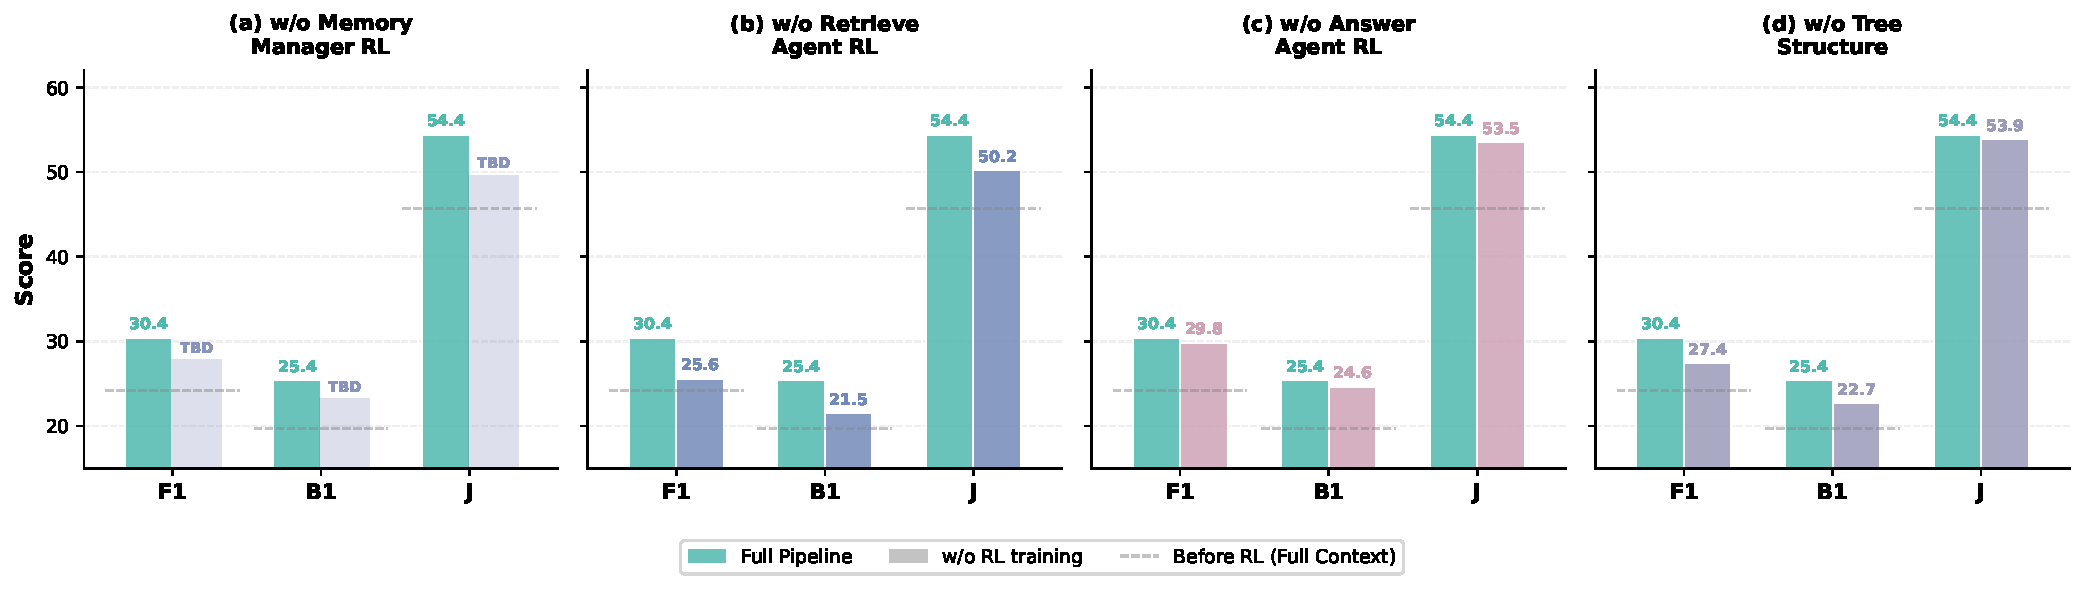
\includegraphics[width=\textwidth]{figures/ablation_figure.pdf}
\caption{Ablation analysis of \textsc{Struct Memory-R1}. Each subfigure shows the effect of disabling RL training for one component: (a) Memory Manager, (b) Retrieve Agent, (c) Answer Agent, and (d) replacing tree structure with flat memory. Teal bars show the full pipeline; colored bars show the ablated variant. Grey dashed lines indicate the before-RL baseline (Full Context). Note that ``w/o'' disables RL fine-tuning for the component, not the component itself. The Memory Manager ablation (hatched bars) is pending completion.}
\label{fig:ablation}
\end{figure}

Figure~\ref{fig:ablation} shows the effect of disabling RL training for each component. Disabling Retrieve Agent RL (Figure~\ref{fig:ablation}b) causes the largest degradation, dropping F1 from 30.4 to 25.6, B1 from 25.4 to 21.5, and J from 54.4 to 50.2. This confirms that learned tree navigation is the most critical component: without it, the system falls back to heuristic retrieval over tree leaves and loses the ability to plan structured search paths.

Disabling Answer Agent RL (Figure~\ref{fig:ablation}c) produces only a modest drop (F1 to 29.8, B1 to 24.6, J to 53.5), suggesting that the base Qwen2.5-3B-Instruct model is already a reasonably capable reader when provided with well-retrieved evidence. The primary bottleneck in our pipeline is retrieval quality, not answer generation.

Replacing tree structure with flat memory (Figure~\ref{fig:ablation}d) while keeping all RL components yields numbers that closely match Memory~R1 (F1 27.4, B1 22.7, J 53.9), as expected since this ablation is architecturally equivalent to Memory~R1. The 3.0-point F1 gap between flat and tree-structured retrieval demonstrates the value of hierarchical memory organization as an inductive bias for the retriever.

The Memory Manager RL ablation (Figure~\ref{fig:ablation}a) is ongoing and will quantify the contribution of RL-trained memory writing.

\section{Discussion}
The results confirm that tree-structured memory provides clear advantages for questions requiring multi-step or temporal reasoning, while flat methods retain an edge on open-domain recall. The 8.6-point F1 gain on multi-hop and 14.1-point gain on temporal questions over Memory~R1 suggest that the hierarchical grouping of facts by speaker, topic, and session enables retrieval paths that flat scoring cannot replicate. At the same time, the dominance of RAG~(BM25) on open-domain questions (39.1 F1) highlights that broad keyword coverage remains valuable when questions do not require structural navigation.

The consistent F1--J divergence across baselines is also informative. Methods that use structured memory (Semantic XPath, our method) tend to achieve higher J relative to their F1, suggesting that tree-guided retrieval surfaces more contextually complete evidence even when the final answer does not lexically match the gold reference. This pattern reinforces the value of evaluating with both lexical and semantic metrics.

The current formulation uses oracle structured data for memory construction, meaning the Memory Manager has not yet been trained end-to-end. This represents an important caveat: the reported gains reflect the ceiling of what tree structure can provide given perfect writing, not what an end-to-end system would achieve. Completing the Memory Manager training loop is the most important next step.

More broadly, the results suggest that structural ambition must be balanced against training stability. The present method uses stable CRUD updates for memory writing, while the Retrieve Agent carries the burden of structure-aware navigation. This division is cleaner than asking a single policy to both reorganize memory arbitrarily and discover retrieval strategies simultaneously.

\section{Limitations}
The present formulation of \textsc{Struct Memory-R1} has three important limitations. First, the Memory Manager does not yet perform general tree restructuring during training; it updates fact memory under a stable induced schema. Second, the Retrieve Agent emits a single search plan rather than acting interactively one level at a time with intermediate observations. Third, the method emphasizes explicit tree search rather than dense vector retrieval, so it does not yet address the hybrid regime in which semantic similarity and structural routing are both learned.

\section{Conclusion}
We introduced \textsc{Struct Memory-R1}, a reinforcement-learning framework that learns tree-structured conversational memory from raw interaction history and decomposes the overall problem into three components: a Memory Manager for writing, a Retrieve Agent for tree search, and an Answer Agent for final response generation. On the LoCoMo benchmark, \textsc{Struct Memory-R1} achieves the highest overall F1 and LLM-judge accuracy among non-oracle methods, with the largest improvements on multi-hop and temporal reasoning where hierarchical memory organization matters most. The framework preserves the central Memory-R1 principle that memory quality should be judged through downstream task performance, while extending it to structure-aware retrieval over induced memory hierarchies. By separating memory construction, retrieval planning, and answer generation, \textsc{Struct Memory-R1} provides a principled path toward long-horizon conversational agents with learned structured memory.

\section{Related Work}
\paragraph{Persistent Memory and RAG.}
Retrieval-augmented generation improves factuality and coverage by accessing external knowledge at inference time~\citep{lewis2020retrieval}. Flat nearest-neighbor memory has likewise been used to improve language-model behavior through direct memory lookup~\citep{khandelwal2020generalization}. In agent settings, memory is often maintained as a chronological stream of observations, reflections, or summaries~\citep{park2023generative}. These approaches demonstrate the value of persistent memory but treat it as a flat collection, without exploiting the event and topic structure inherent in conversation.

\paragraph{RL for Search and Memory.}
Search-R1 treats external search as a policy decision and optimizes reasoning-search trajectories with relative reinforcement learning~\citep{jin2025search}. Memory-R1 extends this perspective to persistent memory, training a Memory Manager and an Answer Agent using downstream question-answering reward~\citep{yan2025memory}. These works establish the key principle that information access and memory manipulation should be trained from task outcomes rather than from heuristic rules. However, Search-R1 addresses external search rather than persistent conversational memory, and Memory-R1 operates over flat memory without addressing tree-structured access or updates. Our work inherits this outcome-driven perspective while extending it to tree-structured memory with learned access and update policies.

\paragraph{Structured Memory Access.}
Structured memory representations expose relations, hierarchies, and subtrees that are unavailable in flat banks. Semantic XPath is representative of work that leverages this structure at inference time by generating path-like queries over memory trees~\citep{semanticxpath2026}. This line of work shows that hierarchical organization can improve memory access, but it typically assumes the structure already exists and relies on heuristic or prompted query generation. Our setting differs in two respects: the tree is induced incrementally from raw conversation, and access over it is optimized as a learned policy using downstream reward.

\paragraph{Gap addressed by this work.}
Prior work treats memory structure, learned access, and learned updates as separate concerns. \textsc{Struct Memory-R1} addresses all three within a unified framework.


\bibliographystyle{plainnat}
\bibliography{reference}

\end{document}
